\documentclass{article} 
\usepackage{tikz}
\usetikzlibrary{decorations.pathreplacing}
\usepackage{xcolor}
\usepackage[a4paper]{geometry}
\usepackage{fancyhdr}
\pagestyle{fancy}
\lhead{Lorentzkraft}
\rhead{September 2025}
\begin{document}
 
\section{Lorentzkraft}
Die Lorentzkraft, $F_L$, ist die Kraft, welche auf elektrisch geladene Teilchen in einem Magnetfeld wirkt.
Die Lorentzkraft, welche auf ein einzelnes Elektron wirkt ist
\[
 F_L = e \cdot v \cdot B
\] 
Auf einen Leiter der Länge $l$ wirkt dabei
\[
 F_L = B \cdot I \cdot l
\]
 
\subsection{\emph{UVW}-Regel} 
Die Richtung der Auswirkung eines Magnetfeldes kann mithilfe \emph{UVW}-Regel bestimmt werden. Dabei wird der Daumen und der Zeige- und Mittelfinger in jeweils $90^\circ$ Winkeln ausgestreckt. Dabei stellt jeder Finger immer die Richtung einer Kraft dar.
\begin{center}
\begin{tabular}{ |l|c|c| }
\hline
 \colorbox{red!30}{U}rsache & Stromfluss & Daumen \\
\hline
 \colorbox{red!30}{V}ermittlung & Magnetfeld & Zeigefinger \\
\hline
 \colorbox{red!30}{W}irkung & Kraft & Mittelfinger \\
\hline
\end{tabular}
\end{center}
Sind zwei Richtungen bekannt, kann diese Regele angewand werden, um die dritte zu finden.
 
\subsection{Messung} 
\begin{minipage}{\dimexpr\linewidth-5cm} 
Zum Messen kann \emph{eine Stromwaage} genutzt werden; ein Messgerät, welches mit einer Waage oder einem Kraftsensor die auf den Leiter wirkende Lorentzkraft misst. Somit kann auch mit der obigen Formel die magnetische Flussdichte bestimmt werden. \newline
Mit den Messdaten können natürlich auch die Proportionalitäten, welche in der Formel aufgefunden werden, begründet werden.
\end{minipage} 
\hfill
\begin{minipage}{5cm}
 \center
 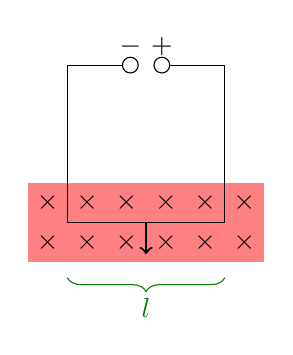
\begin{tikzpicture}
  \fill[red!50] (-1.5, -1.5) rectangle (1.5, -2.5);
  \foreach \x in {-3,...,2} {
   \foreach \y in {0,1} {
    \draw (\x*0.5+0.25, \y*0.5-2.25) node{$\times$};
   };
  };
 
  \draw (-0.2, 0) circle (0.1cm) node[above] {$-$};
  \draw (0.2, 0) circle (0.1cm) node[above] {$+$};
  \draw (-0.3, 0) -- (-1, 0);
  \draw (0.3, 0) -- (1, 0);
  \draw (-1, 0) -- (-1, -2);
  \draw (1, 0) -- (1, -2);  
  \draw (-1, -2) -- (1, -2);
  \draw[->, thick] (0, -2) -- (0, -2.4); 
 
  \draw [green!50!black, decorate,decoration={brace,amplitude=5pt,mirror}]
  (-1,-2.7) -- (1,-2.7) node[midway,below,yshift=-4pt]{$l$};
 \end{tikzpicture} 
\end{minipage} 
\end{document}